%%%%%%%%%% Beamerの初期設定 %%%%%%%%%%%
% beamerを使用する初期設定
\documentclass[aspectratio=169, 12pt, dvipdfmx]{beamer}

% パッケージ読み込み
% 下記のように color / xcolor を追加で読み込む場合は、ドライバオプションは付けずに
\usepackage{graphicx}
\usepackage{lmodern}
\usepackage{amsmath, amssymb, bm,hyperref}
\usepackage{appendixnumberbeamer}
\usepackage{cite}
\usepackage{physics}
\usepackage[version=4]{mhchem}
%デザインの選択 (省略可)
\usetheme{Default}
%%%%%%%%%%%%%%%%%%%%%%%%%%%%%%%%%%%%%


%%%%%%%%%% Beamerの基本的なコード %%%%%%%%%%
% 属性

\title{有限温度におけるSn核の超流動相転移解析\\Woods-Saxonポテンシャルと\\seniority pairingモデルの応用}
\author{根岸 颯}
\date{February 28, 2025} % あるいは特定の日付
\setbeamertemplate{footline}[frame number]
\begin{document}

\begin{frame}
  \titlepage
\end{frame}


\begin{frame}{概要}
  \begin{itemize}
    \item 原子核のエネルギースケールは $1\ \mathrm{MeV} \simeq 10^{10}$ K 程度。
    \item 地上ではこの熱平衡状態は実現せず、通常は $T = 0$ K とみなせる。
    \item しかし、恒星内部や超新星爆発などの極限環境では $T \sim 10^9$ K 以上になり、有限温度の影響を受ける。
    \item 有限温度の原子核の性質は、核融合反応などへの応用が期待される。
    \item 本研究では、\ce{{}^{100-132}Sn} 核を対象に、Woods-Saxon ポテンシャルと seniority pairing モデルを用いた解析を行う。
  \end{itemize}
\end{frame}


\section{理論}

\begin{frame}{Woods-Saxon ポテンシャル}
  \begin{columns}[totalwidth=1.0\linewidth]
    \begin{column}[t]{0.45\linewidth}
      \begin{itemize}
        \item $V(r)=\dfrac{V_0(< 0)}{1+\exp((r-R)/a)}$
        \item より現実的な原子核の性質を反映。
        \item 原子核の密度分布と同じ形状を持つ。
        \item パラメータ:
          \begin{itemize}
            \item \( R \) :原子核の半径
            \item \( a \) :表面のぼやけ
          \end{itemize}
      \end{itemize}
    \end{column}

    \begin{column}[T]{0.55\linewidth}
      \centering
      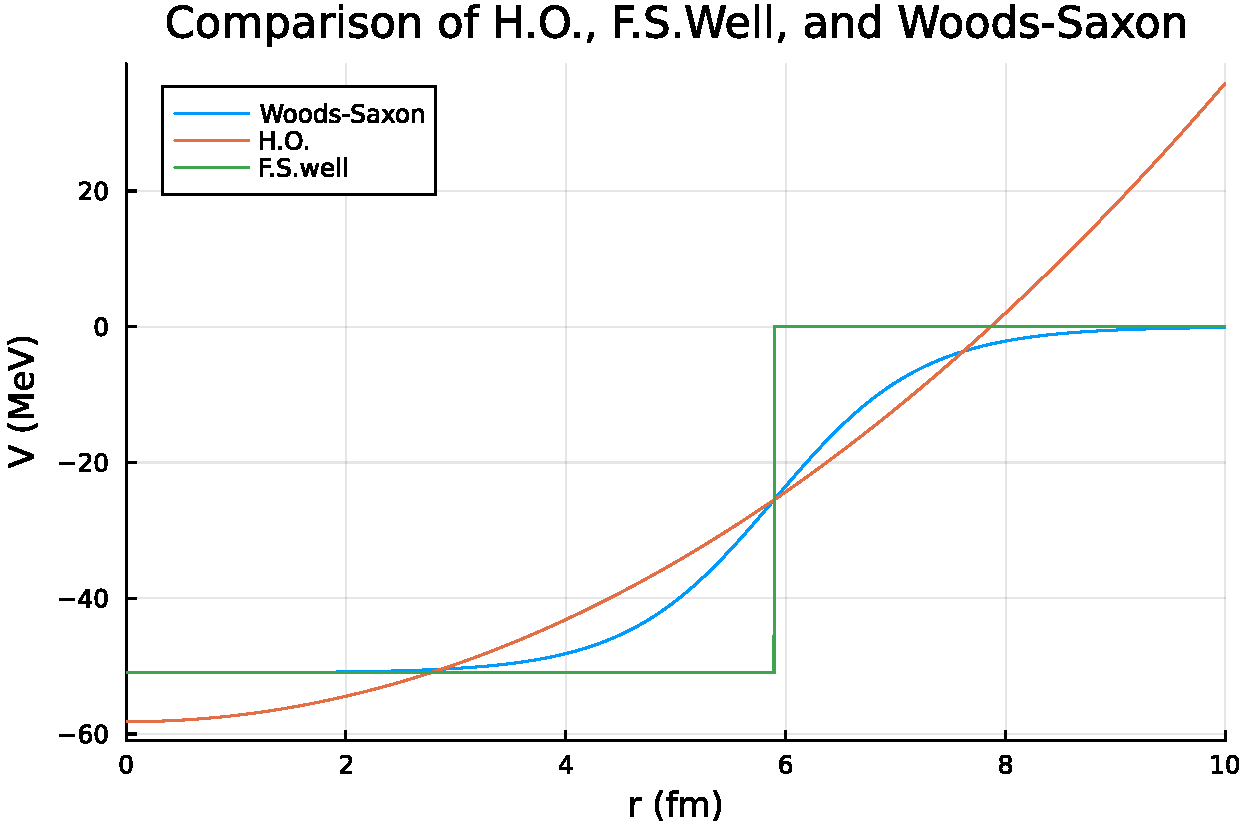
\includegraphics[width=0.9\textwidth]{fig_pdf/Comp_pt.pdf}
      \vspace{5pt}
      \scriptsize \\図1: 各ポテンシャルの比較
    \end{column}
  \end{columns}
\end{frame}


\begin{frame}{平均場近似における単粒子 Hamiltonian}
  \begin{itemize}
    \item Woods-Saxon ポテンシャルを採用し、単粒子 Hamiltonian を定義:
      \[
      H = T_{\text{HO}} + U(r)
      \]
      ここで、\(T_{\text{HO}}\)は  
      \[
      T_{\text{HO}} = \hbar \omega \left( 2n + l + \frac{3}{2} \right)\quad:\hbar\omega=41/A^{-1/3}
      \]
    \item ポテンショル項:
      \[
      U(r) = u_0 f(r) + u_{ls} r_0^2 \frac{1}{r} \frac{df(r)}{dr} \boldsymbol{l} \cdot \boldsymbol{s}
      + U_{\text{Coul}}(r) \frac{1 - \tau}{2}-\frac{1}{2}M\omega^2r^2
      \]
      \[
      f(r) = -\frac{1}{1 + \exp \left( \frac{r - R}{a} \right)}
      \]
    \item この Hamiltonian を対角化し、単粒子エネルギーを求める。
  \end{itemize}
\end{frame}


\begin{frame}{seniority モデルにおける Hamiltonian}
  \begin{itemize}
    \item 残留相互作用を含めた Hamiltonian \( H' \) を、数演算子 \( N_j \) と quasi-spin 演算子 \( S_{j+} \) を用いて定義:
      \[
      H' = \sum_j \epsilon_j N_j - g S_{+} S_{-}
      \]
      ここで、
      \[
      S_{+} \equiv \sum_j S_{j+}, \quad S_{-} \equiv (S_{+})^\dagger
      \]
    \item \( j \) は \( N = 50 \sim 82 \) を満たす軌道を指す。
  \end{itemize}
\end{frame}



%BCS理論の説明。どのような理論なのか、どうして原子核に適用できるのか。
%方程式自体は次のスライドで
\begin{frame}{BCS 理論}
  \begin{itemize}
    \item 引力による対相関では、\( J=0 \) の対が多数の準位に分布。
    \item 多様な分布が可能なため、seniority 数(未ペア粒子数)が低い状態で表されるが、多くの独立状態が存在。
    \item これを説明する理論として、超伝導を記述する BCS 理論が採用される \cite{asakura_structure}(池田、高田)。
    \item 基底状態は変分法的に求められ、超伝導状態として記述される。
    \item BCS 基底状態:
      \[
      \ket{\text{BCS}} = \prod_{k>0} \left( u_k + v_k a^{\dagger}_{k} a^{\dagger}_{\bar{k}} \right) \ket{0}
      \]
  \end{itemize}
\end{frame}

\begin{frame}{BCS 方程式}
  \begin{itemize}
    \item BCS パラメータ \( u_k, v_k \) は、単粒子エネルギー \( \epsilon_k \)、
    化学ポテンシャル \( \lambda \)、ギャップ \( \Delta \) を用いて表される 
    \cite{thenuclearmanybody}(Ring, Schuck):
      \[
      \left.
      \begin{aligned}
        u_k^2\\
        v_k^2
      \end{aligned}
      \right\}
      = \frac{1}{2} \left( 1 \pm \frac{\epsilon_k - \lambda}{\sqrt{(\epsilon_k - \lambda)^2 + \Delta^2}} \right)
      \]
    \item これらのパラメータを決定する方程式:
      \begin{align}
        \Delta  &=  g\sum_{k>0} u_k v_k \quad &\text{(ギャップ方程式)} \label{Gap T=0} \\
        N       &=  2\sum_{k>0} v_k^2 \quad &\text{(粒子数方程式)} \label{number T=0}
      \end{align}
  \end{itemize}
\end{frame}

\begin{frame}{有限温度 BCS 理論1/2}
  文献\cite{goodman1981finite}(Goodman,1981)を参考にした。
  \begin{itemize}
    \item 有限温度では、粒子は熱力学的分布に従い、Fermi 分布:
      \[
      f_i = \frac{1}{1 + \exp(\beta E_i)}
      \]
      を用いる。
    \item ペアリングテンソル\(t\)を求める式:
    %tilde =>  転置,Asterisk =>複素共役, dagger => 随伴
    \[
    t=\tilde{U}fV^* + V^{\dagger}(1-f)U\ \ :
    U=
    \begin{pmatrix}
      u_i & 0 \\
      0 & u_i
    \end{pmatrix},
    V=
    \begin{pmatrix}
      0 & -v_i \\
      v_i & 0
    \end{pmatrix},
    f=
    \begin{pmatrix}
      f_i & 0 \\
      0 & f_i
    \end{pmatrix}
    \]
  \end{itemize}
\end{frame}

\begin{frame}{有限温度 BCS 理論2/2}
  \begin{itemize}
    \item 密度行列を求める式:
    \[
    \rho = \tilde{U}fU^* +V^\dagger(1-f)V
    \]
    \item 以上より、BCS 方程式は以下のように修正される:
      \begin{align}
        \Delta  &=  g\sum_{k>0} u_k v_k (1 - 2 f_k) \quad &\text{(ギャップ方程式)} \label{Gap FT} \\
        N       &=  2\sum_{k>0} \left[ v_k^2 + (u_k^2 - v_k^2) f_k \right] \quad &\text{(粒子数方程式)} \label{number FT} 
      \end{align}
  \end{itemize}
\end{frame}


\begin{frame}{計算手法の概要}
  \begin{itemize}
    \item \textbf{ステップ 1: 単粒子エネルギーの計算}
      \begin{itemize}
        \item Woods-Saxon ポテンシャルを用い、シュレーディンガー方程式を数値的に解く。
        \item 対角化により単粒子準位を求める。
      \end{itemize}
    \item \textbf{ステップ 2: pairing strength $g$ の決定}
      \begin{itemize}
        \item seniority モデルを用い、$g$ を計算。
      \end{itemize}
    \item \textbf{ステップ 3: 有限温度BCS計算}
      \begin{itemize}
        \item ギャップ方程式と粒子数方程式を自己無撞着に解く。
        \item Fermi 分布を導入し、温度依存性を考慮。
      \end{itemize}
  \end{itemize}
\end{frame}

\section{計算手法}
\begin{frame}{ポテンシャルパラメータと波動関数}
  \begin{itemize}
    \item 波動関数は極座標調和振動子波動関数\( \psi_{nlj}\)を採用する。
    \item ポテンショルパラメータ \( u_{0}, u_{ls} \) を設定し、ポテンシャルを決定する。
    \item パラメータ:
      \begin{align}
        r_0 &= 1.27,\quad R = r_0 A^{1/3},\quad a = 0.67 \quad [\text{fm}] \\
        u_0 &= \left(-51+33\dfrac{N-Z}{A}\right),\quad
        u_{ls} = \left(22-14\dfrac{N-Z}{A} \right)\quad [\text{MeV}]
      \end{align}
    \item この波動関数を基底に用い、ハミルトニアンを対角化して単粒子エネルギーを求める。
  \end{itemize}
\end{frame}


%再考してくれ定期
\begin{frame}{ギャップエネルギーの計算}
  \small % フォントサイズを小さくする
  \begin{columns} % 2カラムに分割
    \column{0.6\textwidth} % 左カラム
    \begin{itemize}
      \item 偶奇質量差からギャップエネルギー \( \Delta \) を求める:
        \[
        \Delta = \frac{1}{2} \left( E_{g.s.}^{(N+1)} + E_{g.s.}^{(N-1)} - 2E_{g.s.}^{(N)} \right)
        \]
      \item 基底エネルギーと結合エネルギーの関係:
        \[
        E_{g.s.}^{(N)} = -B(N) + \text{Const.}
        \]
      \item 結合エネルギーの表式:
        \begin{align*}
        B(Z, N) &= a_v A - a_s A^{\frac{2}{3}} - a_A \frac{(N - Z)^2}{A} - a_c \frac{Z^2}{A^{\frac{1}{3}}} \pm \delta\quad:\delta=12/\sqrt{A}
        %体積項、表面積項、対称項、クーロン項、偶奇項
        \end{align*}
    \end{itemize}
    \column{0.3\textwidth} % 右カラム
    \begin{tabular}{c|c}
      Parameter & Value \\ \hline
      \( a_v \) & 15.56 \\
      \( a_s \) & 17.23 \\
      \( a_A \) & 23.285 \\
      \( a_c \) & 0.697 
    \end{tabular}\\
    \scriptsize 表1: 結合エネルギーパラメータ
  \end{columns}
\end{frame}



\begin{frame}{化学ポテンシャルとペアリング強度}
  \begin{itemize}
    \item 化学ポテンシャル \( \lambda \) と pairing strength \( g \) は、BCS 方程式を用いて求める。
    \item 簡単のため、ギャップ \( \Delta_k \) はすべての \( k \) に対して等しいと仮定。
      \begin{align}
        \Delta  &=  \frac{g}{2} \sum_{k>0} \frac{\Delta}{\sqrt{(\epsilon_k - \lambda)^2 + \Delta^2}} \\
        N  &=  \sum_{k>0} \left(1 - \frac{\epsilon_k - \lambda}{\sqrt{(\epsilon_k - \lambda)^2 + \Delta^2}}\right)
      \end{align}
    \item これを満たす \( \lambda, g \) を数値的に求める。
  \end{itemize}
\end{frame}

\begin{frame}{有限温度 BCS 方程式}
  \begin{itemize}
    \item \( T=0 \) の \( g \) を用い、有限温度 BCS 方程式を解く。
    \item ギャップ方程式と粒子数方程式:
      \begin{align}
        \Delta  &=  \frac{g}{2} \sum_{k>0} \Delta\frac{1 - 2 f_i}{\sqrt{(\epsilon_k - \lambda)^2 + \Delta^2}} \\
        N  &=  \sum_{k>0} \left[1 - \frac{(\epsilon_k - \lambda)(1 - 2 f_i)}{\sqrt{(\epsilon_k - \lambda)^2 + \Delta^2}}\right] 
      \end{align}
    \item ここで、Fermi 分布:
      \[
      f_i = \frac{1}{1 + \exp(\beta E_i)}
      \]
  \end{itemize}
\end{frame}

\begin{frame}{エネルギー期待値の計算}
  \begin{itemize}
    \item 温度変化に対するエネルギー期待値:
      \[
      \begin{split}
      \langle H -\lambda N\rangle = \sum_{k>0} \frac{\epsilon_k - \lambda}{2}&\left[
        1 - \frac{\epsilon_k - \lambda}{E_k}\tanh\left(\frac{E_k}{2T}\right)
        \right] \\
        &- \frac{\Delta^2}{G},
      \end{split}
      \]
      \[
        E_k = \sqrt{(\epsilon_k - \lambda)^2 + \Delta^2}.
      \]
    \item ここでも、\( v_k, u_k \) は BCS 方程式の解から求める。
    \item 比熱 \( C \) も温度依存性を評価  (\(H'=H -\lambda N\)):
      \[
      C = \frac{d\langle H' \rangle}{dT}
      \]
  \end{itemize}
\end{frame}


\section{計算結果}

\begin{frame}{$\Delta$の質量数依存性}
  \centering
  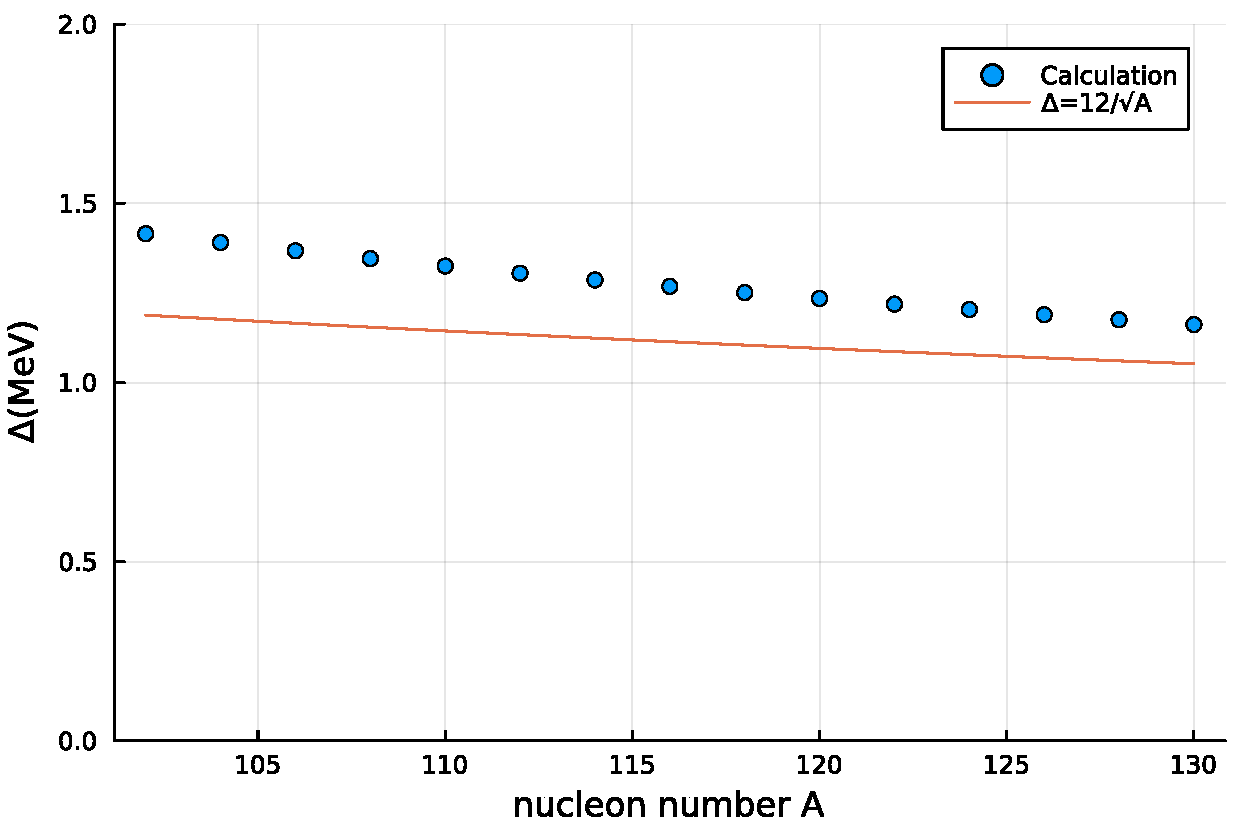
\includegraphics[width=0.5\textwidth]{fig_pdf/Delta_vs_A.pdf}
  \vspace{5pt} % キャプションと画像の間隔調整
  \\
  \scriptsize 図3: $\Delta$と核子数$A$\\
  ここで近似式$\Delta=12A^{-1/2}$は文献\cite{nucleus_structure}(Bohr,Mottelson)より。
\end{frame}

\begin{frame}{pairing gapの温度依存性}
  以下で用いられている\(\Delta_0\)はそれぞれの核種のgapの\(T=0\)での値である。
  \begin{columns}[totalwidth=1.0\linewidth]
    \begin{column}[t]{0.4\linewidth}
      \begin{itemize}
        \item 全核種で相転移が見られた。
        \item $kT/\Delta_0\sim0.55$付近の傾向が見られる。
        \item $\ce{{}^{102}Sn}$のみ例外的な振る舞い。
      \end{itemize}
    \end{column}

    \begin{column}[T]{0.6\linewidth}
      \centering
      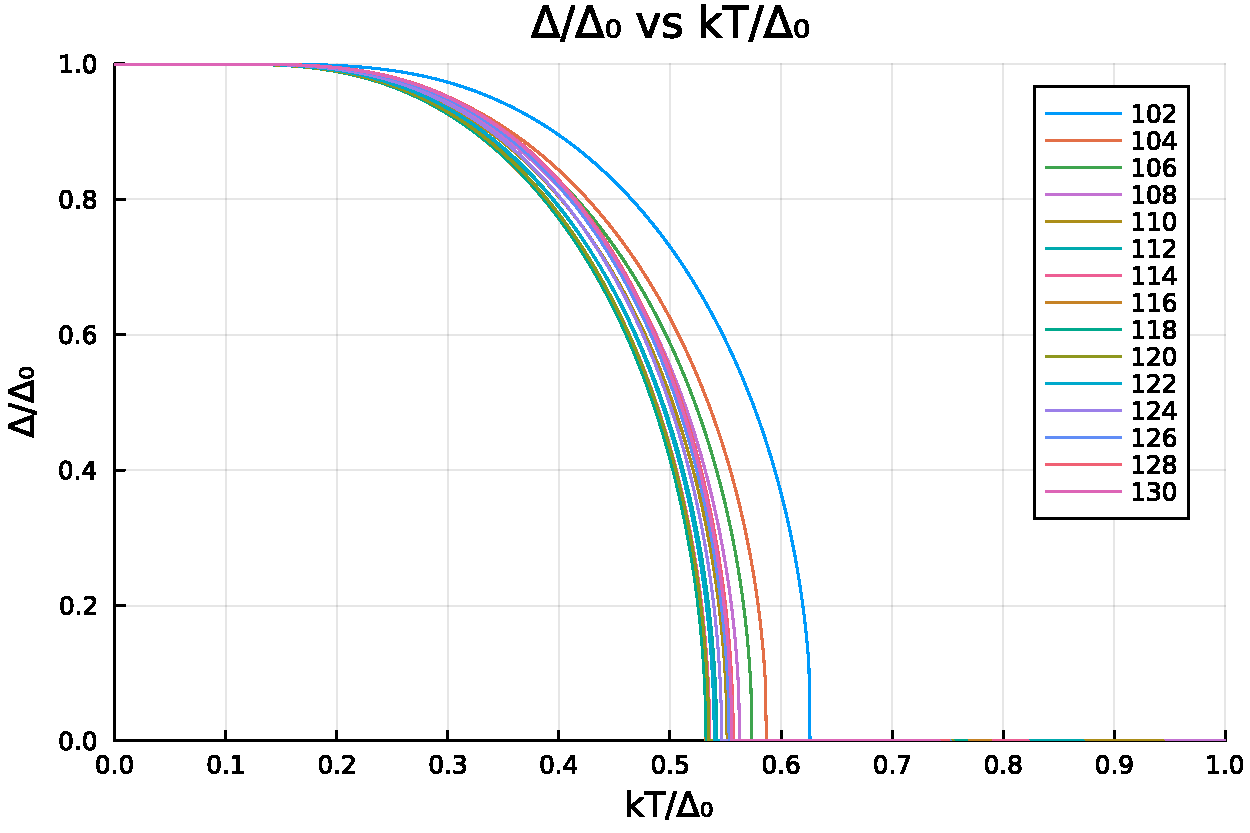
\includegraphics[width=\textwidth]{fig_pdf/Comp_FT_dT.pdf}
      \vspace{5pt} % キャプションと画像の間隔調整
      \scriptsize 図4: pairing gapの温度変化
  \end{column}
  \end{columns}
\end{frame}

\begin{frame}{エネルギーと比熱の温度依存性}
  \begin{columns}[totalwidth=1.0\linewidth]
    \begin{column}[T]{0.48\linewidth}
      \centering
      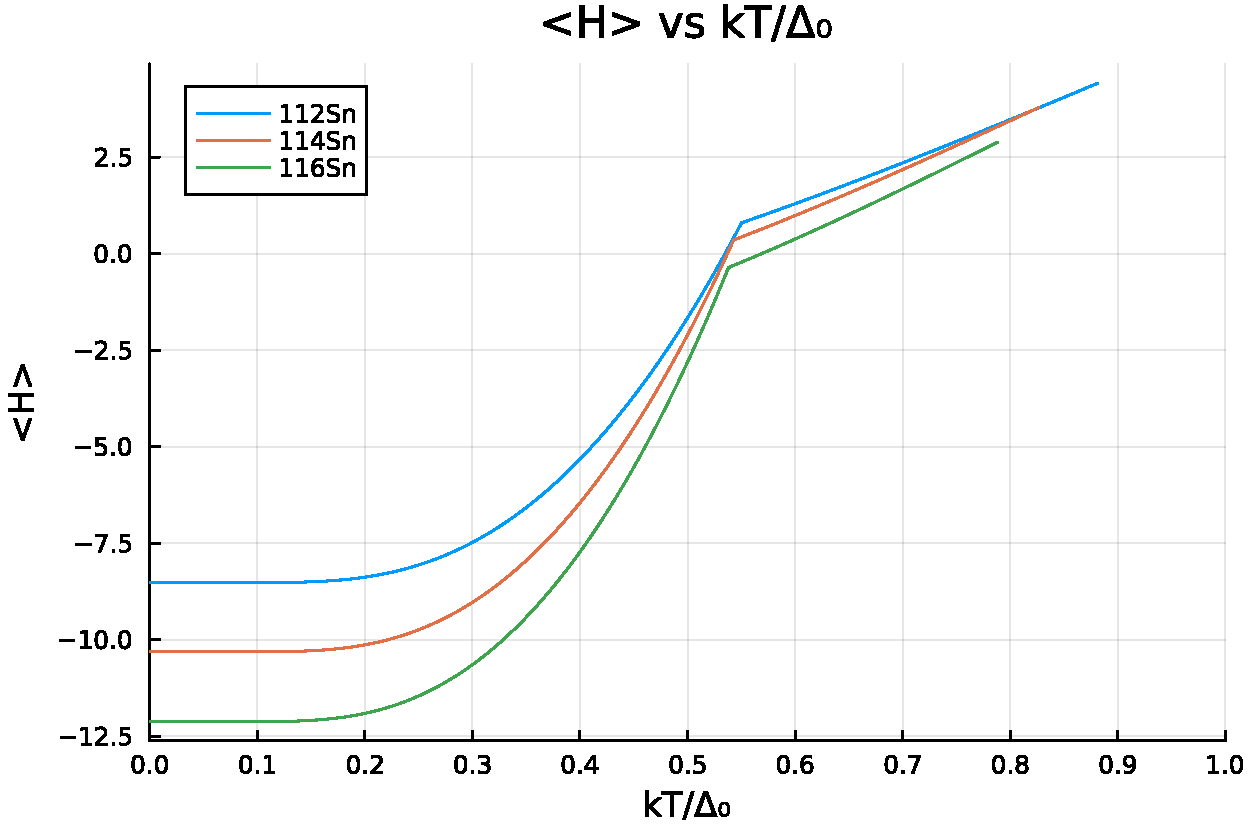
\includegraphics[width=\textwidth]{fig_pdf/Comp_FT_H.pdf}
      \vspace{5pt}
      \scriptsize 図5: エネルギー期待値の温度変化
    \end{column}

    \begin{column}[T]{0.48\linewidth}
      \centering
      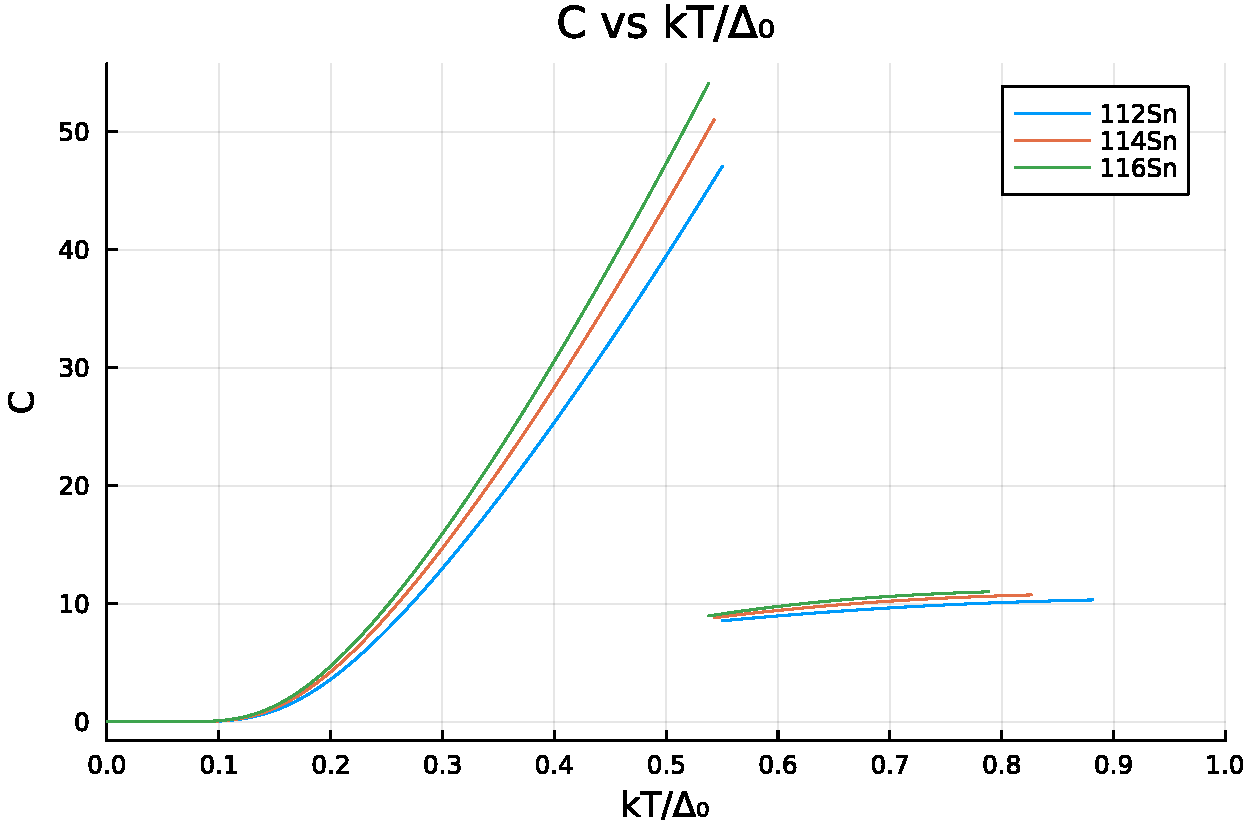
\includegraphics[width=\textwidth]{fig_pdf/Comp_FT_C.pdf}
      \vspace{5pt}
      \scriptsize 図6: 比熱の温度変化
    \end{column}
  \end{columns}
\end{frame}
\section{結論・課題}

\begin{frame}{結論}
  \begin{itemize}
    \item 高温領域で pairing gap の崩壊が確認され、\textbf{相転移} が発生。
    \item エネルギーが上昇すると pairing 効果が弱まり、ギャップが消失。
    \item \textbf{比熱の温度依存性} においても、相転移点付近で急激な変化が見られた。
    \item これらの結果は、超伝導の BCS 理論と類似した傾向を示している。
  \end{itemize}
\end{frame}


\begin{frame}{課題}
  \begin{itemize}
    \item 本解析では Woods-Saxon ポテンシャルと seniority pairing モデルを採用。
    \item これらの手法は計算が容易であるが、以下の簡略化がある:
      \begin{itemize}
        \item 原子核が球対称であると仮定
        \item 同じ \( j \) 殻内の pairing のみを考慮
      \end{itemize}
    \item より現実的な記述のため、以下の発展が期待される:
      \begin{itemize}
        \item 変形核にも対応した計算手法の導入
        \item Gogny 相互作用の採用による相互作用の改良
      \end{itemize}
    \item また、本研究では一粒子励起のみを考慮したが、\textbf{集団励起} との関連も興味深い研究課題である。
  \end{itemize}
\end{frame}


\begin{frame}{参考文献}
  \scriptsize
	\beamertemplatetextbibitems
	\bibliographystyle{junsrt}
  \bibliography{list}
\end{frame}

\texorpdfstring{\appendix}{Appendix}

\begin{frame}{BCS方程式の導出}
  \begin{itemize}
    \item ハミルトニアン:
    \[
      H = 2\sum_{k>0} (\epsilon_k - \lambda) N_k - g S_+ S_-
    \]
    \item 変分法による基底状態(パラメータ\(u_k,v_k\))の決定:
    \[
    \delta\ev**{H}{\text{BCS}}=0
    \]
    \item BCS方程式にパラメータを代入:
    \begin{align}
      \Delta &=g\sum_{k>0}u_k v_k \\
      N      &= 2\sum_{k>0} v_k^2
    \end{align}
  \end{itemize}
\end{frame}

\begin{frame}{有限温度への拡張1/3}
  グランドカノニカル分布によって温度を導入する。
  \begin{itemize}
    \item 自由エネルギーの定義
    \[
    F = \langle H - \lambda N \rangle -TS 
    \]
    \item エントロピーの表現
    \[
    S = -k_B \sum_{k}\left[f_k \ln f_k +(1 -f_k)\ln (1-f_k) \right]
    \]
  \end{itemize}
\end{frame}

\begin{frame}{有限温度への拡張2/3}
  \begin{itemize}
    \item Fermi分布を考慮した方程式
    \[
    f_k = \frac{1}{1+\exp(\beta E_k)}
    \]ここで、\(E_k = \sqrt{(\epsilon_k-\lambda)^2 +\Delta^2}\)
    \item 温度依存性を持つBCS方程式
    \begin{align}
      \Delta &= g\sum_{k>0} u_k v_k(1 -2f_k)\\
      N      &= 2\sum_{k>0} \left[v_k^2 + (u_k^2-v_k^2)f_k\right]
    \end{align}
  \end{itemize}
\end{frame}

\begin{frame}{有限温度への拡張3/3 その1}
  \begin{itemize}
    \item ハミルトニアンの表式
    \[
      H'=\sum_{k}(\epsilon_k - \lambda)a^{\dagger}_ka_k
    \]
    \[
      -g\sum_{kk'>0}a^{\dagger}_{k}a^{\dagger}_{\bar{k'}}a_{\bar{k'}}a_{k}
    \]
  \end{itemize}
\end{frame}

\begin{frame}{有限温度への拡張3/3 その2}
  \begin{itemize}
    \item 個数演算子の期待値\( \langle a^{\dagger}_k a_k \rangle \):
    \[
      \langle a^{\dagger}_k a_k \rangle = v_k^2 + (u_k^2 -v_k^2)f_k
    \]
  \end{itemize}
\end{frame}

\begin{frame}{自由エネルギーとエントロピーの温度依存性}
  \begin{columns}[totalwidth=1.0\linewidth]
    \begin{column}[T]{0.5\linewidth}
      \centering
      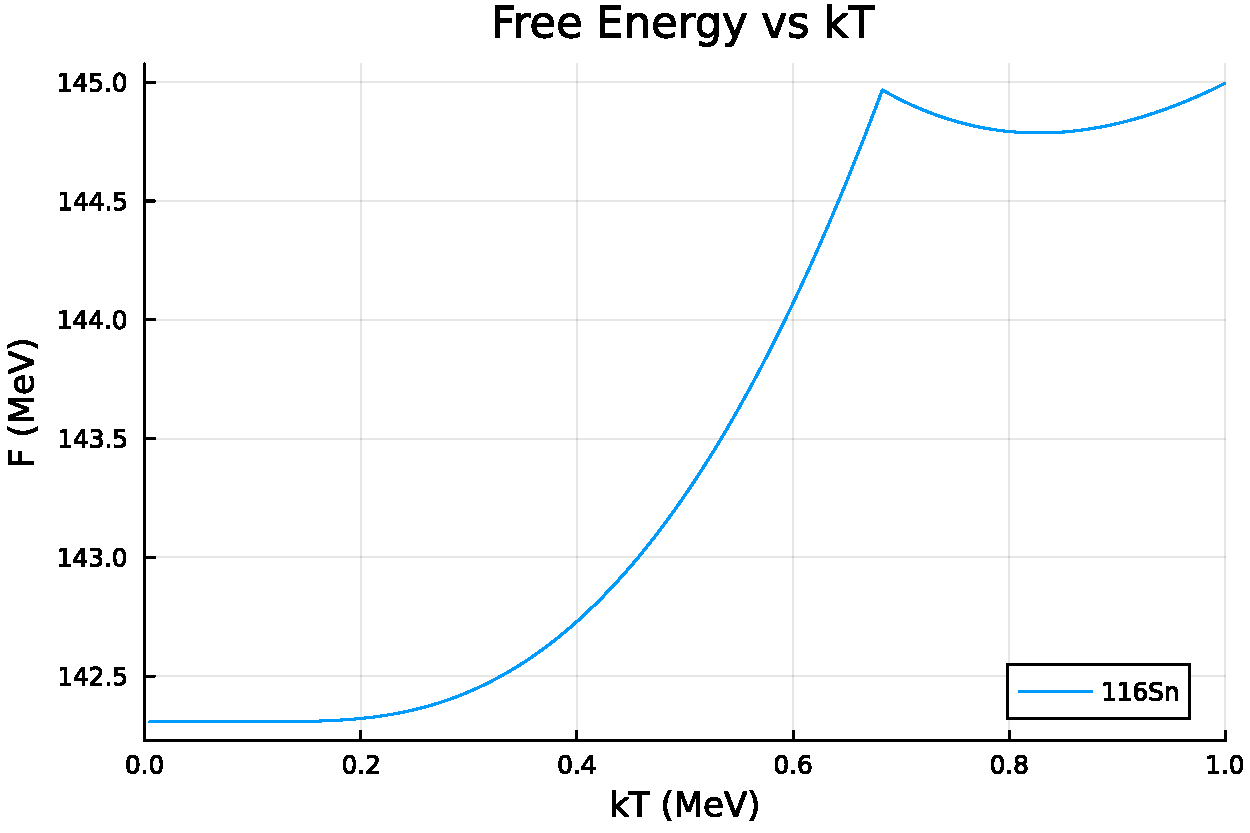
\includegraphics[width=\textwidth]{fig_pdf/F_vs_kT.pdf}
      \vspace{5pt} % キャプションと画像の間隔調整
      \scriptsize 図7: 自由エネルギーの温度変化
    \end{column}

  \begin{column}[T]{0.5\linewidth}
    \centering
    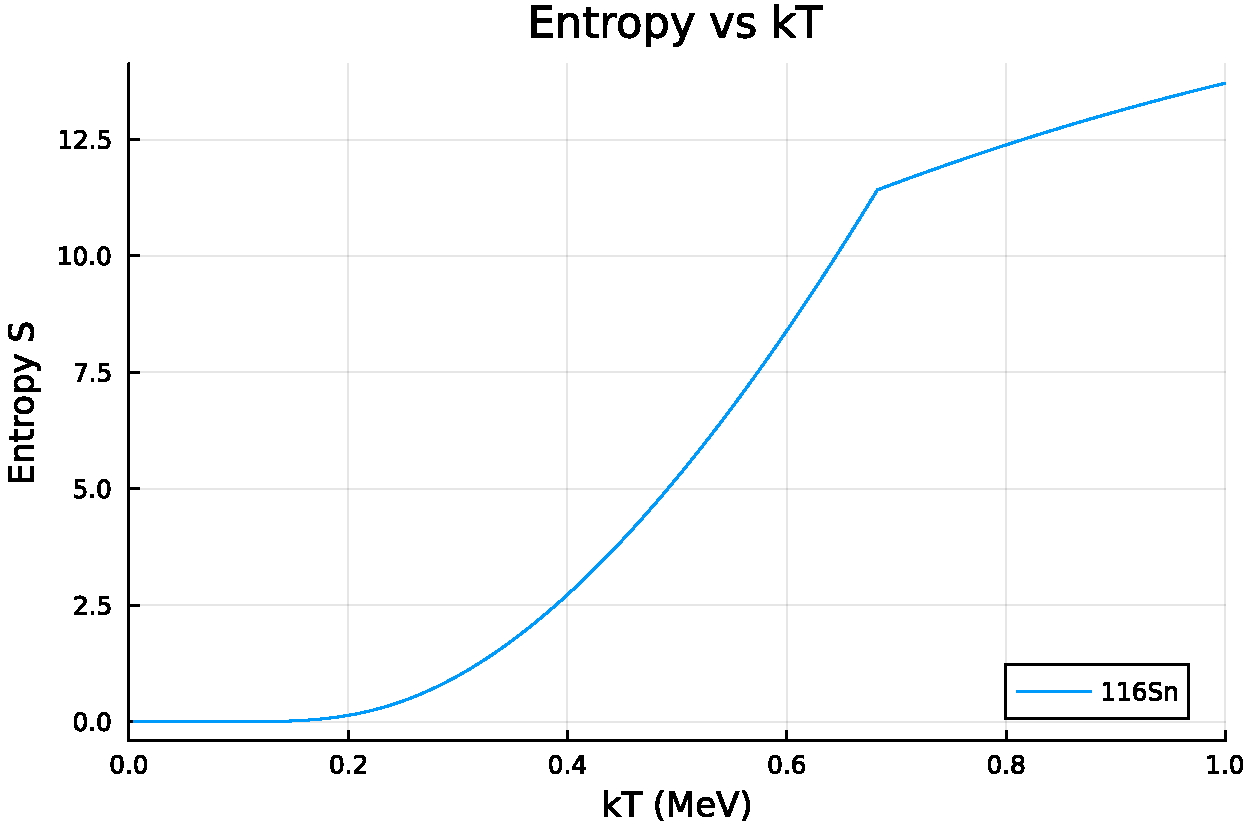
\includegraphics[width=\textwidth]{fig_pdf/S_vs_kT.pdf}
    \vspace{5pt} % キャプションと画像の間隔調整
    \scriptsize 図8: エントロピーの温度変化
  \end{column}
  \end{columns}
\end{frame}

\begin{frame}{他の核種における温度変化}
  \centering
  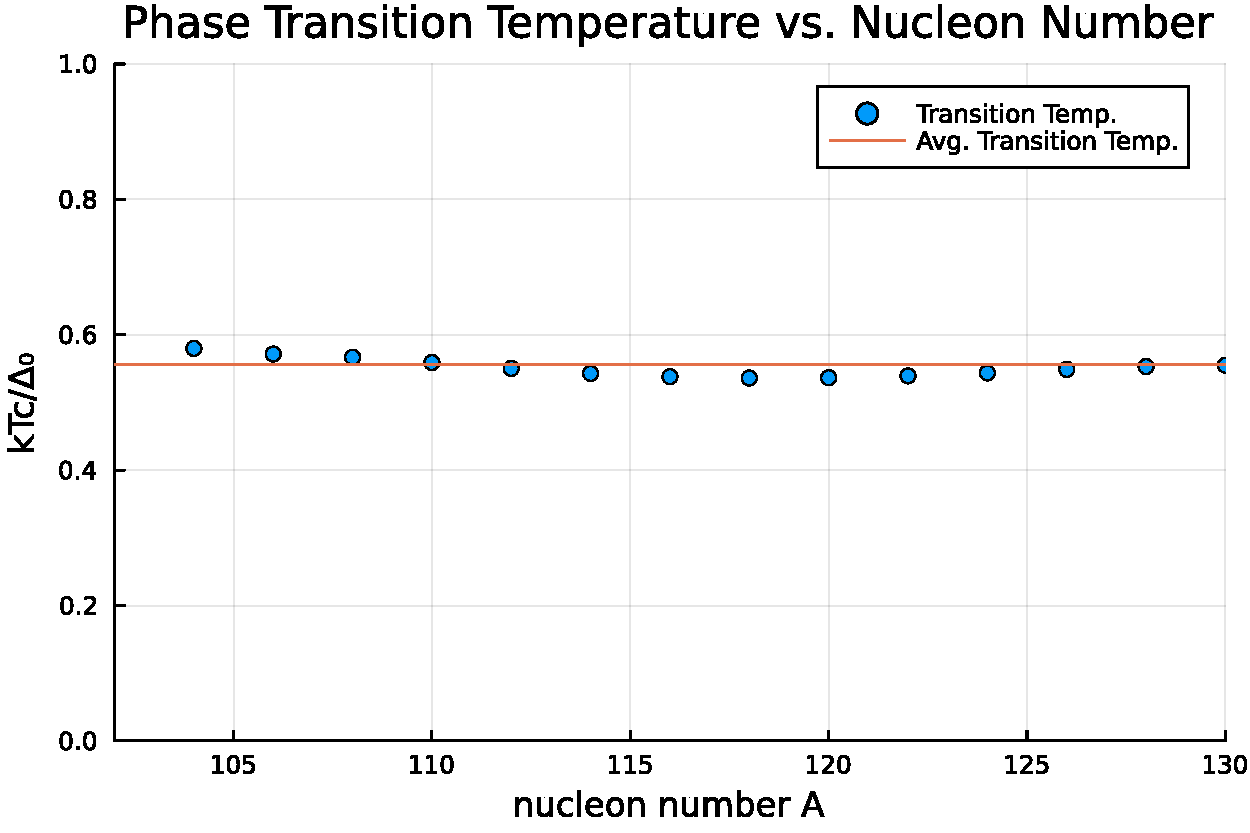
\includegraphics[width=0.5\textwidth]{fig_pdf/A_kT.pdf}
  \vspace{5pt} % キャプションと画像の間隔調整
  \\
  \scriptsize 図9: 相転移温度$k_BT_c$と核子数$A$\\
\end{frame}

\begin{frame}{全核種の相転移温度}
  以下にはギャップ方程式が非自明な解\(\Delta \neq 0\)が消失する温度を示す。
  \centering
  \begin{tabular}{c|c || c|c}
    核種 & \(k_B T_C\) & 核種 & \(k_B T_C\) \\
    \hline
    $\mathrm{{}^{102}Sn}$ & 0.30535 MeV & $\mathrm{{}^{116}Sn}$ & 0.6826 MeV \\
    $\mathrm{{}^{104}Sn}$ & 0.39563 MeV & $\mathrm{{}^{118}Sn}$ & 0.70309 MeV \\
    $\mathrm{{}^{106}Sn}$ & 0.47009 MeV & $\mathrm{{}^{120}Sn}$ & 0.71904 MeV \\
    $\mathrm{{}^{108}Sn}$ & 0.53269 MeV & $\mathrm{{}^{122}Sn}$ & 0.73118 MeV \\
    $\mathrm{{}^{110}Sn}$ & 0.58351 MeV & $\mathrm{{}^{124}Sn}$ & 0.74009 MeV \\
    $\mathrm{{}^{112}Sn}$ & 0.6242 MeV & $\mathrm{{}^{126}Sn}$ & 0.74631 MeV \\
    $\mathrm{{}^{114}Sn}$ & 0.6567 MeV & $\mathrm{{}^{128}Sn}$ & 0.7503 MeV \\
    & & $\mathrm{{}^{130}Sn}$ & 0.75242 MeV
  \end{tabular}
  \vspace{5pt}\\
  \scriptsize 表2: 核種ごとの相転移温度$k_B T_c$\\
\end{frame}

\end{document}
